% Template for FMI-2011 paper; to be used with:
%          fmiconf.sty - LaTeX style file, and
%          IEEEbib.bst - IEEE bibliography style file.
% --------------------------------------------------------------------------
\documentclass{article}
\usepackage{fmiconf,amsmath,epsfig}

\usepackage{german}
\usepackage[utf8]{inputenc}
\usepackage{url}

% Example definitions.
\def\x{{\mathbf x}}
\def\L{{\cal L}}

% Title.
\title{Kann eine Drohne präzise nur mit den Sensoren eines Smartphones gesteuert werden?}
\name{Stefan Baumann, Florian Gümbel}
\address{Technische Hochschule Mittelhessen}

\begin{document}
\maketitle
\begin{abstract}
Drohne ist mittlerweile ein fest etablierter Begriff, der ein von vier Propellern und Elektromotor angetriebenes Flugobjekt beschreibt. Die Steuerung erfolgt zumeist über eine Anwendung auf Smartphone / Tablet. Dabei wird hauptsächlich ein virtueller Joystick auf dem Bildschirm angezeigt der mit Gesten gesteuert wird.\\ Eine andere aber bisher aber weitestgehend eingeschränkt genutzte Art der Steuerung ist der Einsatz von Hilfe Gyro- und Bewegungssensor des Smartphones. Eingeschränkt insofern, als dass nicht alle Möglichkeiten der Sensoren genutzt werden. An diesem Ansatz soll mit der Entwicklung einer nativen Android App für Smartphones angeknüpft werden. Ziel ist es, die Bewegungen, die vom Benutzer mit dem Smartphone getätigt werden, an die Drohne zu übertragen. Zusätzlich sollen Gesten das Steuern von Foto- und Vieoaufnahmen und deren Übertragung auf das Display des Smartphones vervollständigen.\\ Am Ende gilt es die Frage zu beantworten, ob die Steuerung einer Drohne präzise genug ist, wenn diese komplett auf Gyroskop und Accelerometer des Smartphones gekoppelt ist.

\end{abstract}

\section{Einleitung}
\label{sec:einleitung}
Immer mehr erfreuen sich sogenannte Drohnen an Beliebtheit. Diese neue Form des unbemannten Flugobjekte zeichnet sich zumeist dadurch aus, dass sie, anders als herkömmliche bekannte Modellflugzeuge, mindestens vier kleine Propeller hat welche über Elektromotoren angetrieben werden und die Drohne senkrecht starten lassen. Die Anzahl der Propeller kann variieren. Angefangen von Quadrocopter über Hexacopter und Octacopter bis hin zu Multicopter. Der Einsatzzweck einer solchen Drohne geht von Vermessungstechnik über Luftaufnahmen und Erkundung bis hin zur Jagd.

Um eine Solche Drohne zu Steuern gibt es verschiedene Möglichkeiten. Abhängig von Modell lassen sich klassische Fernsteuerungen entweder direkt mit der Drohne Verbinden oder über Umweg mit Hilfe einer App. Nahezu jeder Drohnenhersteller bietet eine eigene App für alle gängigen Smartphones oder Tablets an. Die Verbindung findet je nach Modell über W-Lan oder Bluetooth statt. Für die Steuerung mittels App auf dem Gerät steht ein digitaler Joystick zur Verfügung dessen Bewegung umgerechnet und auf die Drohne Übertragen wird während das Gerät ruhig in der Hand liegt. Meistens wird über den linken Joystick die vertikale Bewegung gesteuert. Dazu zählt die Veränderung Höhe und die Drehung in beide Richtungen. Der Rechte Joystick ist für die horizontale Bewegung zuständig. Damit ist das Schwenken zur Seite sowie das Vorwärts- und Rückwärtsfliegen gemeint. 
\ Die Idee ist es nun, eine weitere Möglichkeit zu untersuchen, bei der zwei Sensoren des Smartphones für die Steuerung zum Einsatz kommen. Dabei soll anstelle der Bedienung auf dem Touchscreen das gesamte Gerät als Steuerungseinheit genutzt werden. \\Gyroskop und Accelerometer dienen zur Erfassung der Bewegungen und das Smartphone überträgt die diese auf die Drohne. Zusätzlich sollen Gesten weitere Funktionen zur Verfügung stellen. Dazu zählen unter anderem das Aufnehmen von Fotos und Videos.
\begin{figure}[htb]
\begin{minipage}[b]{1.0\linewidth}
  \centering
\centerline{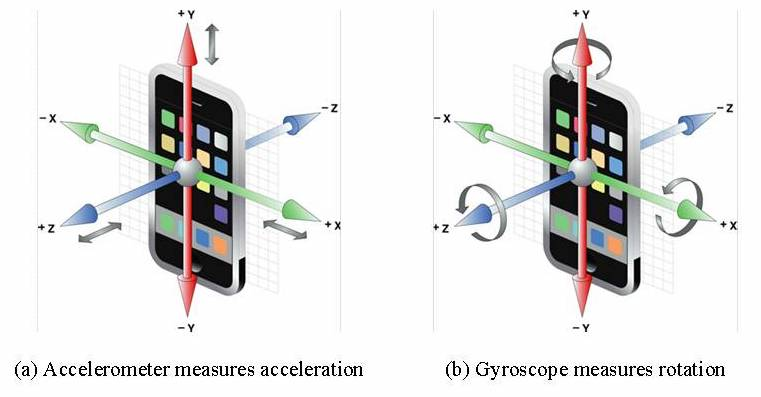
\includegraphics[width= 85mm]{gyro.jpg}}
\end{minipage}
\caption{Accelerometer und Gyrosensor}
\label{fig:gyro}
\end{figure}


\section{Verwandte Arbeiten}
\label{sec:verwandteArbeiten}
Derzeit gibt es nicht nur Hersteller eigenen Anwendungen zum Steuern einer Drohne sondern bereits eine Vielzahl von Drittanbietersoftware. 
\\ Eine davon ist die hauseigenen Anwendung AR.FreeFlight des Drohnenherstellers Parrot \footnote{https://play.google.com/store/apps/details?id=com.parrot.freeflight\&hl=de}, die Steuerung durch Neigung unterstützt. Allerdings wird durch die Neigung nur die Flugrichtung bestimmt und nicht der gesamte Steuerungsprozess. Das eigentliche Fliegen geschieht mit Joystick-ähnlichen Bedienelementen auf dem Display. \\Bereits Anfang 2015 hat Sony ein Projekt vorgestellt, in dem eine Drohne mittels SmartWatch 2, SmartEyeglass und Smartphone gesteuert wird\footnote{http://developer.sonymobile.com/2015/01/05/control-a-mini-drone-with-smarteyeglass-and-smartwatch-2-tutorial/}. In diesem Fall ist die SmartWatch via Bluetooth mit dem Smartphone verbunden und überträgt die Bewegung per W-Lan an die Drohne. Über das Dsiplay der Smartwatch lassen sich dabei die verschiedenen Steuerungs-Modi umschalten.

\section{Methodik}
Beschreibung des Vorgehens
Unterteilung in logische abschnitte
konzept / verfahrensvergleiche / analyse MEthodenauswahl
implementierung / erinscrämungen / realisierung
\section{Ergebnisse und Evaluation}

\section{Zusammenfassung und Ausblick}
\bibliography{Template}{}
\bibliographystyle{IEEEbib}
\end{document}